\documentclass{beamer}
\usepackage[serbianc]{babel}
\usepackage{graphicx}
\usepackage{makeidx}
\makeindex
\usefonttheme{professionalfonts}
\usetheme{CambridgeUS}

\title{Основе веб програмирања}
\author{Борисав Живановић (borisavz)}

\begin{document}

    \begin{frame}
        \maketitle
    \end{frame}

    \section{Садржај}

    \begin{frame}{Садржај}
        \begin{enumerate}
            \item Основни појмови мрежног програмирања
            \item Клијент-сервер архитектура
            \item Еволуција веб апликација
            \item HTTP протокол
            \item Рад са базом података
            \item Архитектура веб апликације
            \item Аутентификација и ауторизација
        \end{enumerate}
    \end{frame}

    \section{Основни појмови мрежног програмирања}
    \subsection{Packet switching}

    \begin{frame}[allowframebreaks]{Packet switching}
        \begin{itemize}
            \item Потребно је да поруку пошаљемо примаоцу
            \item Директна веза са сваким примаоцем није остварива
            \item Идеја: повезивање пошиљаоца/примаоца у мрежу, дељење комуникационог канала
            \item Решење: \textbf{комутација пакета (packet switching)}
            \begin{itemize}
                \item Поруку изделимо на пакете
                \item Пакетима додамо заглавље (header) са адресом пошиљаоца и примаоца
                \item Систем зна путање до примаоца
                \item Поруку шаљемо пакет по пакет
                \item Само један пакет заузима комуникациони канал
                \item Пакети могу да путују различитим путањама кроз мрежу, да дођу у различитом редоследу до примаоца, или да нестану
            \end{itemize}
        \end{itemize}

        \framebreak

        \begin{figure}
            \centering
            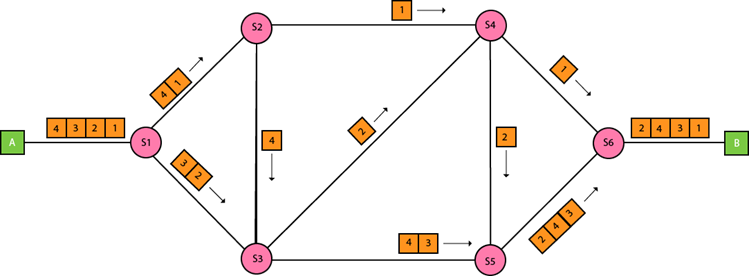
\includegraphics[width=0.75\textwidth]{images/pcsw.png}
            \caption{комутација пакета (packet switching)}
            \label{fig:pcsw}
        \end{figure}
    \end{frame}

    \subsection{IP, DNS}

    \begin{frame}[allowframebreaks]{Internet Protocol}
        \begin{itemize}
            \item Како би комуницирали у мрежи, потребно је да сваки учесник у комуникацији има додељену \textbf{јединствену} адресу
            \item Поруци придружујемо \textbf{заглавље (header)} које садржи:
            \begin{itemize}
                \item Адресу пошиљаоца (source address)
                \item Адресу примаоца (destination address)
                \item Додатна поља (верзија IP протокола, flags, TTL, checksum, ...)
            \end{itemize}
            \item Захваљујући овом заглављу систем зна коме да проследи поруку
            \item У одговори су адресе пошиљаоца и примаоца \textbf{замењене}!
        \end{itemize}

        \framebreak

        \begin{figure}
            \centering
            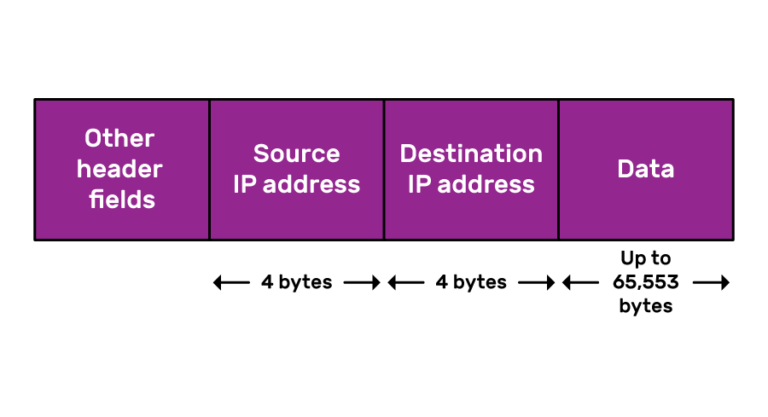
\includegraphics[width=0.75\textwidth]{images/ip.png}
            \caption{упрошћена структура IP пакета}
            \label{fig:ip}
        \end{figure}
    \end{frame}

    \begin{frame}[allowframebreaks]{DNS}
        \begin{itemize}
            \item Проблем: све више сервера на мрежи
            \item Није практично памтити сваку адресу у бројчаном облику
            \item Идеја: систем за придруживање имена, сличан телефонском именику
            \item Решење: \textbf{DNS (Domain Name System)}
            \begin{itemize}
                \item IP адреси додељујемо симболичко име (домен)
                \item Домени су хијерархијски (структура стабла)
                \item DNS је одговоран за одређени део хијерархије
                \item Као одговор враћа IP адресу или адресу одговорног DNS сервера
                \item Морамо знати IP адресу DNS сервера!
            \end{itemize}
        \end{itemize}

        \framebreak

        \begin{figure}
            \centering
            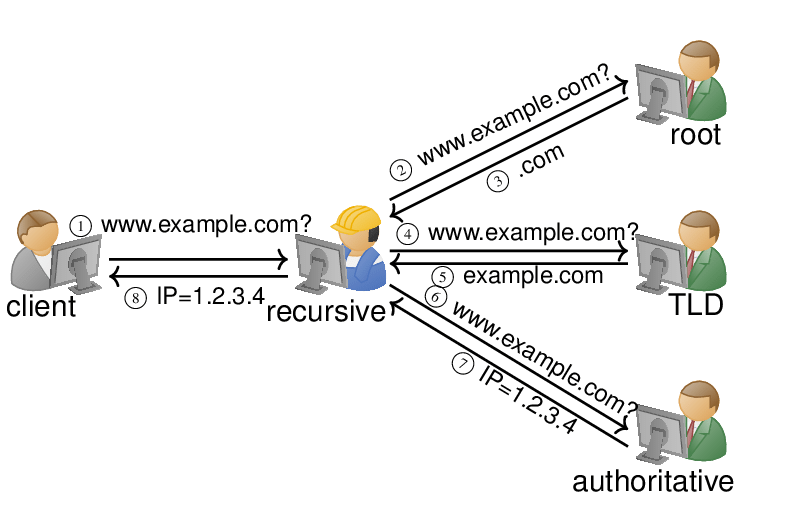
\includegraphics[width=0.75\textwidth]{images/dns.png}
            \caption{DNS упит}
            \label{fig:dns}
        \end{figure}
    \end{frame}
    
    \subsection{TCP, UDP}
    
    \begin{frame}[allowframebreaks]{Transmission Control Protocol}
        \begin{itemize}
            \item Решили смо проблем адресирања уређаја на мрежи...
            \item ...али нисмо проблеме редоследа пристиглих пакета и нестајања пакета
            \item Додатни проблем: шта ако имамо више мрежних апликација на истом рачунару, како да проследимо поруку одговарајућој апликацији?
        \end{itemize}
        
        \framebreak
        
        \begin{itemize}
            \item Решење: \textbf{TCP (Transmission Control Protocol)}
            \begin{itemize}
                \item Додајемо додатно заглавље на нашу поруку
                \item Заглавље садржи source и destination port (слично адреси пошиљаоца и примаоца, али се односи на апликацију), sequence number (редослед поруке)
                \item Уколико пакет нестане, шаље се поново
                \item Оперативни систем осигурава да само једна апликација користи одређени порт
            \end{itemize}
        \end{itemize}
        
        \framebreak
        
        \begin{figure}
            \centering
            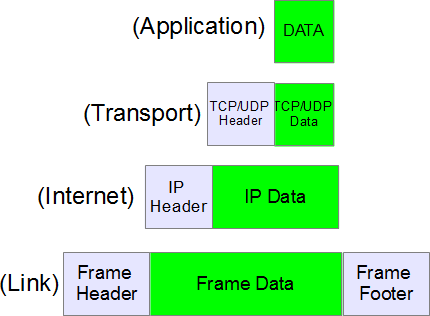
\includegraphics[width=0.6\textwidth]{images/enc.png}
            \caption{енкапсулација пакета}
            \label{fig:tcp_enc}
        \end{figure}
        
        \framebreak
        
        \begin{figure}
            \centering
            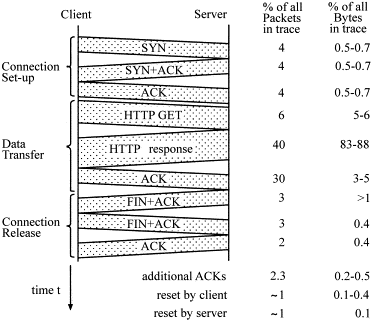
\includegraphics[width=0.5\textwidth]{images/tcp_http.png}
            \caption{Ток TCP комуникације}
            \label{fig:tcp_flow}
        \end{figure}
    \end{frame}
    
    \begin{frame}[allowframebreaks]{User Datagram Protocol}
        \begin{itemize}
            \item Успостављање конекције траје одређено време
            \item За поруке које стају у један пакет, можемо користити једноставнији \textbf{UDP (User Datagram Protocol)}
            \item Задржавамо адресирање апликација, али губимо гаранцију испоруке
            \item DNS користи UDP
        \end{itemize}
    
        \framebreak
        
        \begin{figure}
            \centering
            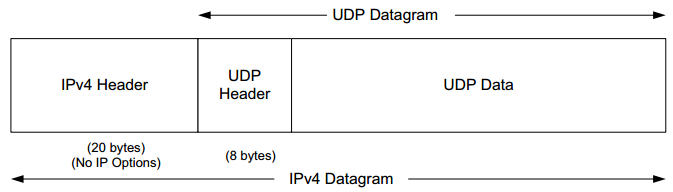
\includegraphics[width=0.75\textwidth]{images/udp_enc.png}
            \caption{енкапсулација пакета}
            \label{fig:udp_enc}
        \end{figure}
        
        \framebreak
        
        \begin{figure}
            \centering
            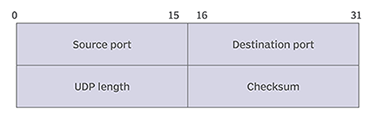
\includegraphics[width=0.75\textwidth]{images/udp_header.png}
            \caption{Садржај заглавља}
            \label{fig:udp_header}
        \end{figure}
    \end{frame}

\end{document}
